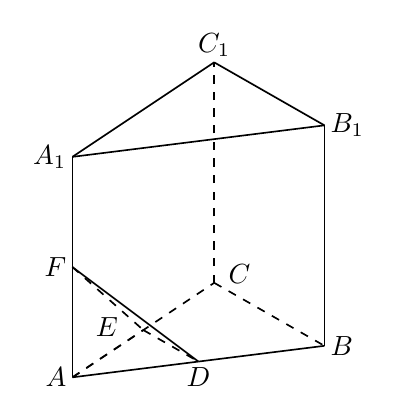
\begin{tikzpicture}[x=1cm,y=1cm,font=\normalsize,
  edge/.style={draw=black,solid,line width=.6pt},
  hide/.style={draw=black,dashed,line width=.6pt}]
% Triangular prism A1B1C1-ABC; D,E,F midpoints of AB,AC,AA1
\coordinate (A) at (0.0,0.0);
\coordinate (B) at (3.2,0.4);
\coordinate (C) at (1.8,1.2);
\coordinate (A1) at (0.0000000000,2.8000000000);
\coordinate (B1) at (3.2000000000,3.2000000000);
\coordinate (C1) at (1.8000000000,4.0000000000);
\coordinate (D) at (1.6,0.2);
\coordinate (E) at (0.9,0.6);
\coordinate (F) at (0.0000000000,1.4000000000);
% solid outline
\draw[edge] (A1)--(B1);
\draw[edge] (B1)--(B);
\draw[edge] (B)--(D);
\draw[edge] (D)--(A);
\draw[edge] (A1)--(F);
\draw[edge] (F)--(D);
\draw[edge] (A1)--(C1);
\draw[edge] (B1)--(C1);
% hidden edges and small section triangle
\draw[edge] (F)--(A);
\draw[hide] (A)--(C);
\draw[hide] (C)--(B);
\draw[hide] (C)--(C1);
\draw[hide] (A)--(E);
\draw[hide] (E)--(D);
\draw[hide] (F)--(E);
\node[left,inner sep=2pt] at (A) {$A$};
\node[right,inner sep=2pt] at (B) {$B$};
\node[right,inner sep=2pt,xshift=3pt,yshift=3pt] at (C) {$C$};
\node[left,inner sep=2pt] at (A1) {$A_{1}$};
\node[right,inner sep=2pt] at (B1) {$B_{1}$};
\node[above,inner sep=2pt] at (C1) {$C_{1}$};
\node[below,inner sep=2pt] at (D) {$D$};
\node[left,inner sep=2pt,xshift=-7pt,yshift=1pt] at (E) {$E$};
\node[left,inner sep=2pt] at (F) {$F$};
\end{tikzpicture}
